\documentclass[english,10pt,a4paper,twocolumn,colorscheme=green]{orarticle}
\usepackage{hyperref}
\usepackage{bbm}

\usepackage{listings}
\lstset{
	language=C++,
	commentstyle=\color{darkgreen}\textit,
	frame=single,
	tabsize=4,
	keywordstyle=\color{blue}\bfseries,
	stringstyle=\color[gray]{0.4},
	basicstyle=\lst@ifdisplaystyle\scriptsize\else\ttfamily\fi,
	morekeywords={uint16, uint32, Vec2, Vec3}
}

\begin{document}

	\titlehead{\begin{minipage}{0.5\linewidth}
		\begin{center}
		Otto-von-Guericke-University Magdeburg\\
		Faculty of Computer Science\\
		ISG - Computational Visualistics
		\end{center}
	\end{minipage}}
%	\subject{File Format Documentation}
	\title{Fitting Minimal Bounding Ellipsoids}
	\authors{Johannes Jendersie}
	\abstract{Abstract}{
		Building a bounding volume hierarchy with axis aligned ellipsoids can be done with different fitting strategies. One could search the Löwner-John ellipsoid for the convex hull of the geometry in a subtree. This is complicated and relatively slow depending on the build method. I purpose an approximative and iterative solution which uses two operations: fit an ellipsoid with known center and a single point and fit an ellipsoid to two given ellipsoids.
	}
	\thispagestyle{empty}
	\maketitle
	
	
	% ************************************************************************ %
	\section{Minimal Ellipsoid}
	There are multiple representations of the ellipsoid: implicit (also in matrix form) and parametric.
	\begin{align}
	\left\lVert\frac{\mathbbm{x}-\mathbbm{c}}{\mathbbm{a}}\right\rVert &= 1\\
	(\mathbbm{x}-\mathbbm{c})^T diag(\mathbbm{a}) (\mathbbm{x}-\mathbbm{c}) &= 1\\
	\mathbbm{a}\cdot\begin{pmatrix}
		\cos(u) \cos(v)\\
		\cos(u) \sin(v)\\
		\sin(u)
	\end{pmatrix} &= \mathbbm{x}
	\end{align}
	where $\mathbbm{c}$ is the center and $\mathbbm{a}$ is the vector of radii. Each vector operation inclusive the division is component-wise.
	
	The minimal ellipsoid is usually defined as the ellipsoid of minimal volume:
	\begin{align}
		V = \frac{4}{3}\pi \prod_{i=1}^d \mathbbm{a}_i
	\end{align}
	In degenerated cases where some of the radii are 0, which may happen if fitting ellipsoids to axis aligned triangles, the volume becomes 0 too. In that case the minimal ellipses (smallest) area is searched.
	
	% ************************************************************************ %
	\section{Point and Center Known}
	
	Finding a minimal ellipsoid with a known center $\mathbbm{a}$ to contain a point is equivalent to find the minimal ellipsoid to a symmetric box with that point as one corner and the same center.
	
	\begin{figure}[h]
	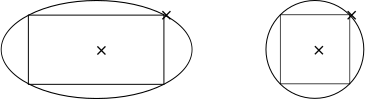
\includegraphics[width=\linewidth]{img/ellipsoidpointfitting}
	\caption{Finding the best ellipsoid for a point is equivalent to that of a symmetric box. On the right side the space is rescaled such that the ellipsoid becomes a sphere.}
	\end{figure}
	The optimal bounding sphere for a cube with side length $s$ has $r = s\frac{\sqrt{3}}{2}$. The $\sqrt{3}$ comes from the euclidean length from the center to one corner $\sqrt{3\cdot\frac{s^2}{2^2}}$. In the general case for $d$ dimensions the factor is $\frac{\sqrt{d}}{2}$. In case of an ellipsoid the only difference is that the space must be scaled first which happens when use a vector of three side lengths $2\lvert\mathbbm{x}-\mathbbm{c}\rvert$ instead of $s$. In the degenerated case where one or more of that lengths are 0 the factor shrinks.
	\begin{align}
		\mathbbm{a} = \lvert\mathbbm{x}-\mathbbm{c}\rvert\cdot\sqrt{\sum_{i=1}^d (\mathbbm{x}_i-\mathbbm{c}_i) \neq 0}
	\end{align}
	
	\textbf{Proof} There are infinite many ellipsoid through the given point, which can be computed as:
	\begin{align*}
		\left\{\mathbbm{a}_0, \mathbbm{a}_1, \sqrt{\frac{(\mathbbm{x}_2-\mathbbm{c}_2)^2}{1-\frac{\mathbbm{x}_0-\mathbbm{c}_0}{\mathbbm{a}_0}^2 - \frac{\mathbbm{x}_1-\mathbbm{c}_1}{\mathbbm{a}_1}^2}}\right\}
	\end{align*}
	where $\mathbbm{a}_0, \mathbbm{a}_1$ can be chosen freely.
	W.l.o.g. an ellipsoid with $\mathbbm{a}_0 - \epsilon$ which again contains the point $\mathbbm{x}$ has a larger volume than the proposed solution.
	
	\begin{align*}
		V(\mathbbm{a}) &< V(\mathbbm{a}')\\
		s_i &= \lvert \mathbbm{x}_i-\mathbbm{c}_i \rvert\\
		\mathbbm{a}_0 \cdot\mathbbm{a}_1 \cdot\mathbbm{a}_2 &< (\mathbbm{a}_0-\epsilon) \cdot\mathbbm{a}_1 \cdot\sqrt{\frac{s_2^2}{1-\frac{s_0}{\mathbbm{a}_0-\epsilon}^2 - \frac{s_1}{\mathbbm{a}_1}^2}}\\	
		3\cdot s_0\cdot s_2 &< (\mathbbm{a}_0-\epsilon) \cdot\sqrt{\frac{s_2^2}{1-\frac{s_0}{\mathbbm{a}_0-\epsilon}^2 - \frac{1}{\sqrt{3}}}}\\
		9\cdot s_0^2 &< (\sqrt{3}\cdot s_0-\epsilon)^2 \cdot\frac{1}{1-\frac{s_0}{\sqrt{3}s_0-\epsilon}^2 - \frac{1}{\sqrt{3}}}\\
		9-\frac{9}{\sqrt{3}}\cdot s_0^2 &- 9 \cdot \frac{s_0^4}{(\sqrt{3}s_0-\epsilon)^2} < (\sqrt{3}\cdot s_0-\epsilon)^2\\
	%	(\sqrt{3}\cdot s_0-\epsilon)^2 &\cdot (1-\frac{1}{\sqrt{3}}\cdot s_0^2) - s_0^4 < \frac{(\sqrt{3}\cdot s_0-\epsilon)^4}{9}\\
	\end{align*}
	
	Well I don't see how to simplify this... but testing it seemed ok.
	
\end{document}